\documentclass{article}

\usepackage{graphicx}

\newcommand{\Nif}{\rm $^{56}$Ni }

\begin{document}
\title{Plots for the $M_{ej}$ correlations}
\maketitle

%%##TO ADD TEXT
This document has the plots for the ejecta mass calculations using the measured NIR light curves of CSP-I objects. It also includes a short discussion of the distributions in the literature or from complementary methods.

\begin{itemize}

\item \Nif mass using Arnett's rule and $t_0$ using the Jeffrey 1999 formalism

\item \Nif mass from the nebular phase line and the ejecta mass from Scalzo et al 2014 relation (using the stretch values)

\item Calculated from Richard's MCMC

\end{itemize}


\begin{figure}
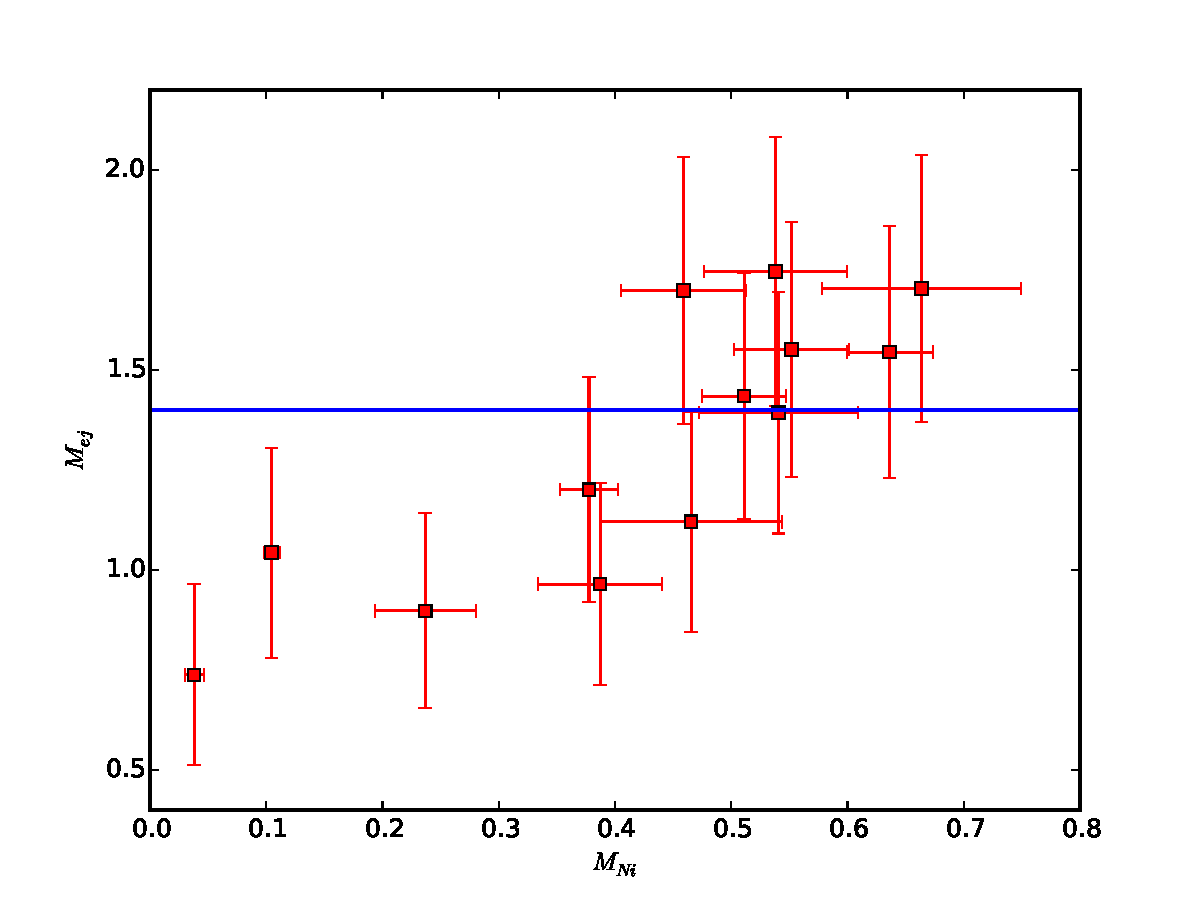
\includegraphics[width=.5\textwidth, trim = 0 0 30 30]{mej_mni_risetime.pdf}
\caption{Using a variable rise time for the Nickel mass calculations, the relation between M$_{ej}$- \Nif mass}
\label{fig:mej-mni}
\end{figure}

\begin{figure}
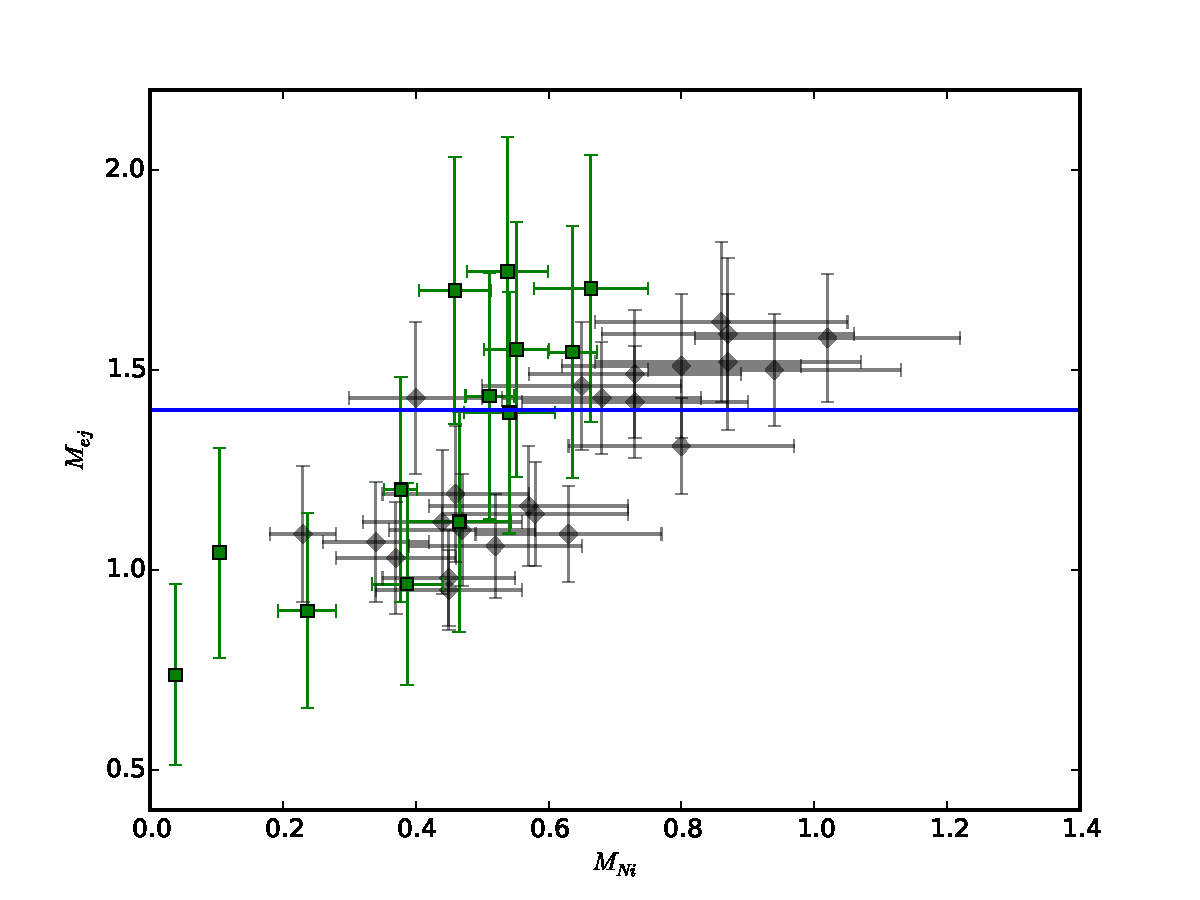
\includegraphics[width=.5\textwidth, trim = 0 0 30 30]{mej_mni_richard_comparison.pdf}
\caption{Comparing the SNe in Figure~\ref{fig:mej-mni} to the calculations by Richard}
\end{figure}

Richard's sample doesn't include fast-decliners and uses the Bayesian framework.
\end{document}




